\documentclass{standalone}
\usepackage{tikz}
\usetikzlibrary{patterns, positioning}


\begin{document}
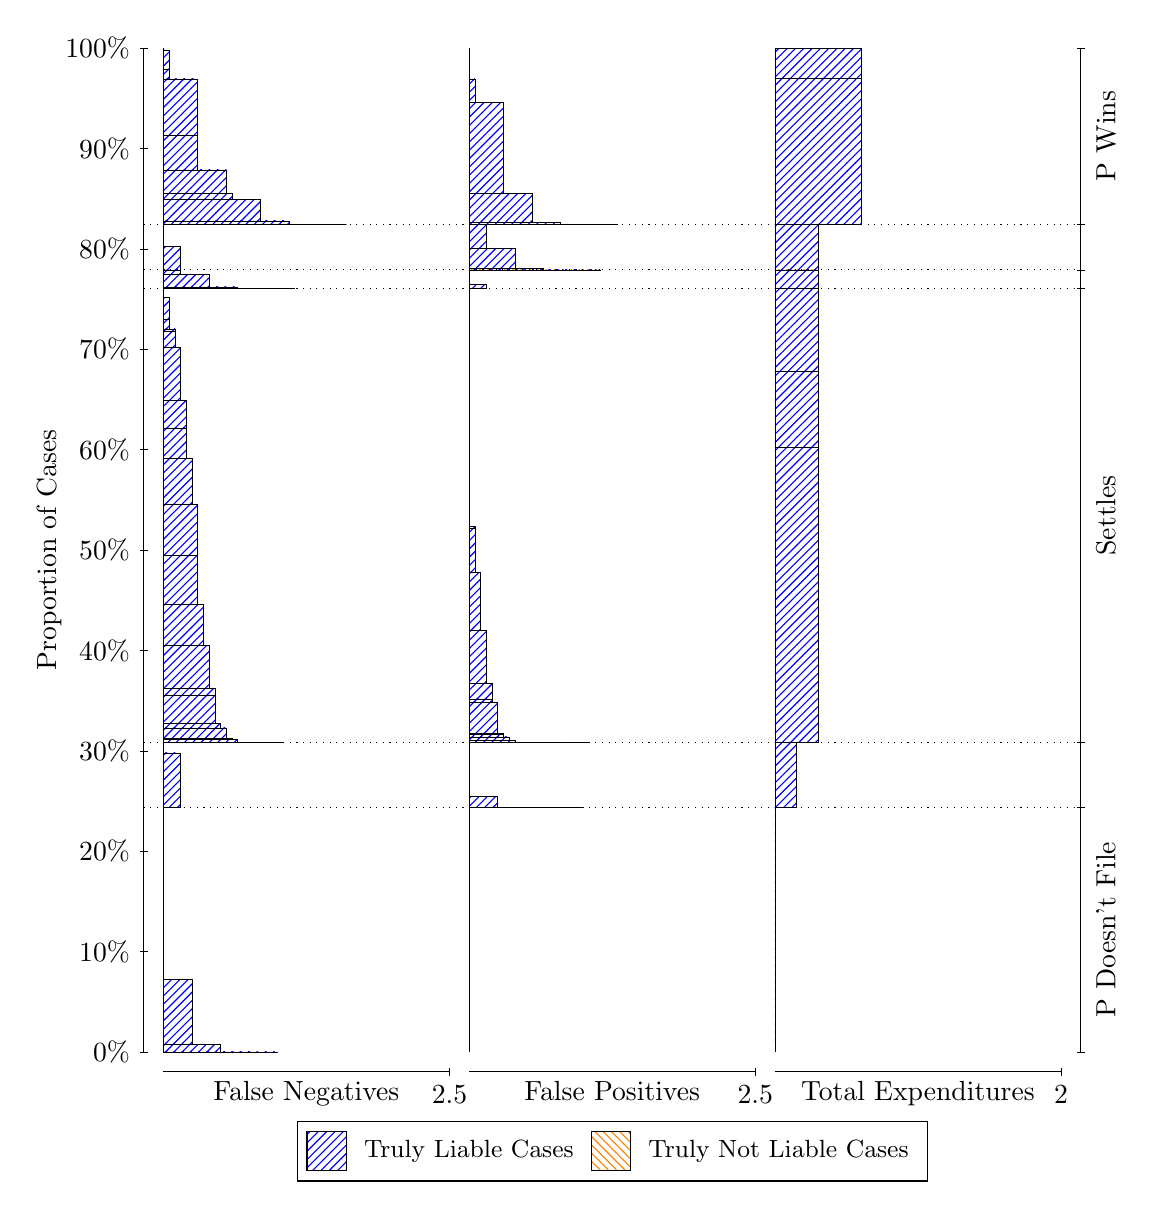
\begin{tikzpicture}
\draw[black, very thin] (1.5,1.75) -- (1.5,14.5);
\node[rotate=90, text=black, anchor=center] at (0.3, 8.125) {Proportion of Cases};
\draw[black, very thin] (1.45,1.75) -- (1.55,1.75);
\node[text=black, anchor=east] at (1.45, 1.75) {0\%};
\draw[black, very thin] (1.45,3.025) -- (1.55,3.025);
\node[text=black, anchor=east] at (1.45, 3.025) {10\%};
\draw[black, very thin] (1.45,4.3) -- (1.55,4.3);
\node[text=black, anchor=east] at (1.45, 4.3) {20\%};
\draw[black, very thin] (1.45,5.575) -- (1.55,5.575);
\node[text=black, anchor=east] at (1.45, 5.575) {30\%};
\draw[black, very thin] (1.45,6.85) -- (1.55,6.85);
\node[text=black, anchor=east] at (1.45, 6.85) {40\%};
\draw[black, very thin] (1.45,8.125) -- (1.55,8.125);
\node[text=black, anchor=east] at (1.45, 8.125) {50\%};
\draw[black, very thin] (1.45,9.4) -- (1.55,9.4);
\node[text=black, anchor=east] at (1.45, 9.4) {60\%};
\draw[black, very thin] (1.45,10.675) -- (1.55,10.675);
\node[text=black, anchor=east] at (1.45, 10.675) {70\%};
\draw[black, very thin] (1.45,11.95) -- (1.55,11.95);
\node[text=black, anchor=east] at (1.45, 11.95) {80\%};
\draw[black, very thin] (1.45,13.225) -- (1.55,13.225);
\node[text=black, anchor=east] at (1.45, 13.225) {90\%};
\draw[black, very thin] (1.45,14.5) -- (1.55,14.5);
\node[text=black, anchor=east] at (1.45, 14.5) {100\%};

\draw[black, very thin] (13.4,1.75) -- (13.4,14.5);
\draw[black, very thin] (13.35,1.75) -- (13.45,1.75);
\node[anchor=west] at (13.35, 1.75) {};
\draw[black, very thin] (13.35,4.8575) -- (13.45,4.8575);
\node[anchor=west] at (13.35, 4.8575) {};
\draw[black, very thin] (13.35,5.6822) -- (13.45,5.6822);
\node[anchor=west] at (13.35, 5.6822) {};
\draw[black, very thin] (13.35,11.448) -- (13.45,11.448);
\node[anchor=west] at (13.35, 11.448) {};
\draw[black, very thin] (13.35,11.682) -- (13.45,11.682);
\node[anchor=west] at (13.35, 11.682) {};
\draw[black, very thin] (13.35,12.262) -- (13.45,12.262);
\node[anchor=west] at (13.35, 12.262) {};
\draw[black, very thin] (13.35,14.5) -- (13.45,14.5);
\node[anchor=west] at (13.35, 14.5) {};

\draw[black, very thin, pattern color=blue, pattern=north east lines] (1.75,1.75) rectangle (3.2033,1.75);
\draw[black, very thin, pattern color=blue, pattern=north east lines] (1.75,1.75) rectangle (2.84,1.7508);
\draw[black, very thin, pattern color=blue, pattern=north east lines] (1.75,1.7508) rectangle (2.4767,1.8511);
\draw[black, very thin, pattern color=blue, pattern=north east lines] (1.75,1.8511) rectangle (2.1133,2.6734);
\draw[black, very thin, pattern color=orange, pattern=north west lines] (1.75,2.6734) rectangle (1.75,2.6734);
\draw[black, very thin, pattern color=blue, pattern=north east lines] (1.75,2.6734) rectangle (1.75,4.8575);
\draw[black, very thin, pattern color=blue, pattern=north east lines] (1.75,4.8575) rectangle (1.968,5.5472);
\draw[black, very thin, pattern color=orange, pattern=north west lines] (1.75,5.5472) rectangle (1.75,5.5472);
\draw[black, very thin, pattern color=blue, pattern=north east lines] (1.75,5.5472) rectangle (1.75,5.6822);
\draw[black, very thin, pattern color=blue, pattern=north east lines] (1.75,5.6822) rectangle (3.276,5.6822);
\draw[black, very thin, pattern color=blue, pattern=north east lines] (1.75,5.6822) rectangle (3.1307,5.6822);
\draw[black, very thin, pattern color=blue, pattern=north east lines] (1.75,5.6822) rectangle (2.9853,5.6823);
\draw[black, very thin, pattern color=blue, pattern=north east lines] (1.75,5.6823) rectangle (2.9127,5.6823);
\draw[black, very thin, pattern color=blue, pattern=north east lines] (1.75,5.6823) rectangle (2.84,5.6825);
\draw[black, very thin, pattern color=blue, pattern=north east lines] (1.75,5.6825) rectangle (2.7673,5.6827);
\draw[black, very thin, pattern color=blue, pattern=north east lines] (1.75,5.6827) rectangle (2.6947,5.7207);
\draw[black, very thin, pattern color=blue, pattern=north east lines] (1.75,5.7207) rectangle (2.622,5.7365);
\draw[black, very thin, pattern color=blue, pattern=north east lines] (1.75,5.7365) rectangle (2.5493,5.8651);
\draw[black, very thin, pattern color=blue, pattern=north east lines] (1.75,5.8651) rectangle (2.4767,5.9206);
\draw[black, very thin, pattern color=blue, pattern=north east lines] (1.75,5.9206) rectangle (2.404,6.2812);
\draw[black, very thin, pattern color=blue, pattern=north east lines] (1.75,6.2812) rectangle (2.404,6.367);
\draw[black, very thin, pattern color=blue, pattern=north east lines] (1.75,6.367) rectangle (2.3313,6.9092);
\draw[black, very thin, pattern color=blue, pattern=north east lines] (1.75,6.9092) rectangle (2.2587,7.4386);
\draw[black, very thin, pattern color=blue, pattern=north east lines] (1.75,7.4386) rectangle (2.186,8.0525);
\draw[black, very thin, pattern color=blue, pattern=north east lines] (1.75,8.0525) rectangle (2.186,8.7082);
\draw[black, very thin, pattern color=blue, pattern=north east lines] (1.75,8.7082) rectangle (2.1133,9.2914);
\draw[black, very thin, pattern color=blue, pattern=north east lines] (1.75,9.2914) rectangle (2.0407,9.6769);
\draw[black, very thin, pattern color=blue, pattern=north east lines] (1.75,9.6769) rectangle (2.0407,10.026);
\draw[black, very thin, pattern color=blue, pattern=north east lines] (1.75,10.026) rectangle (1.968,10.703);
\draw[black, very thin, pattern color=blue, pattern=north east lines] (1.75,10.703) rectangle (1.8953,10.897);
\draw[black, very thin, pattern color=blue, pattern=north east lines] (1.75,10.897) rectangle (1.8953,10.933);
\draw[black, very thin, pattern color=blue, pattern=north east lines] (1.75,10.933) rectangle (1.8227,11.056);
\draw[black, very thin, pattern color=blue, pattern=north east lines] (1.75,11.056) rectangle (1.8227,11.338);
\draw[black, very thin, pattern color=blue, pattern=north east lines] (1.75,11.338) rectangle (1.75,11.339);
\draw[black, very thin, pattern color=orange, pattern=north west lines] (1.75,11.339) rectangle (1.75,11.339);
\draw[black, very thin, pattern color=blue, pattern=north east lines] (1.75,11.339) rectangle (1.75,11.448);
\draw[black, very thin, pattern color=blue, pattern=north east lines] (1.75,11.448) rectangle (3.4213,11.448);
\draw[black, very thin, pattern color=blue, pattern=north east lines] (1.75,11.448) rectangle (3.058,11.448);
\draw[black, very thin, pattern color=blue, pattern=north east lines] (1.75,11.448) rectangle (2.6947,11.467);
\draw[black, very thin, pattern color=blue, pattern=north east lines] (1.75,11.467) rectangle (2.3313,11.626);
\draw[black, very thin, pattern color=blue, pattern=north east lines] (1.75,11.626) rectangle (1.968,11.682);
\draw[black, very thin, pattern color=orange, pattern=north west lines] (1.75,11.682) rectangle (1.75,11.682);
\draw[black, very thin, pattern color=blue, pattern=north east lines] (1.75,11.682) rectangle (1.968,11.985);
\draw[black, very thin, pattern color=orange, pattern=north west lines] (1.75,11.985) rectangle (1.75,11.985);
\draw[black, very thin, pattern color=blue, pattern=north east lines] (1.75,11.985) rectangle (1.75,12.262);
\draw[black, very thin, pattern color=blue, pattern=north east lines] (1.75,12.262) rectangle (4.0753,12.262);
\draw[black, very thin, pattern color=blue, pattern=north east lines] (1.75,12.262) rectangle (3.712,12.262);
\draw[black, very thin, pattern color=blue, pattern=north east lines] (1.75,12.262) rectangle (3.3487,12.305);
\draw[black, very thin, pattern color=blue, pattern=north east lines] (1.75,12.305) rectangle (3.276,12.305);
\draw[black, very thin, pattern color=blue, pattern=north east lines] (1.75,12.305) rectangle (2.9853,12.577);
\draw[black, very thin, pattern color=blue, pattern=north east lines] (1.75,12.577) rectangle (2.9127,12.582);
\draw[black, very thin, pattern color=blue, pattern=north east lines] (1.75,12.582) rectangle (2.622,12.654);
\draw[black, very thin, pattern color=blue, pattern=north east lines] (1.75,12.654) rectangle (2.5493,12.952);
\draw[black, very thin, pattern color=blue, pattern=north east lines] (1.75,12.952) rectangle (2.2587,12.952);
\draw[black, very thin, pattern color=blue, pattern=north east lines] (1.75,12.952) rectangle (2.186,13.392);
\draw[black, very thin, pattern color=blue, pattern=north east lines] (1.75,13.392) rectangle (2.186,14.109);
\draw[black, very thin, pattern color=blue, pattern=north east lines] (1.75,14.109) rectangle (1.8953,14.109);
\draw[black, very thin, pattern color=blue, pattern=north east lines] (1.75,14.109) rectangle (1.8227,14.226);
\draw[black, very thin, pattern color=blue, pattern=north east lines] (1.75,14.226) rectangle (1.8227,14.476);
\draw[black, very thin, pattern color=orange, pattern=north west lines] (1.75,14.476) rectangle (1.75,14.476);
\draw[black, very thin, pattern color=blue, pattern=north east lines] (1.75,14.476) rectangle (1.75,14.5);
\draw[black, very thin, pattern color=orange, pattern=north west lines] (5.6333,1.75) rectangle (5.6333,1.75);
\draw[black, very thin, pattern color=blue, pattern=north east lines] (5.6333,1.75) rectangle (5.6333,4.8575);
\draw[black, very thin, pattern color=orange, pattern=north west lines] (5.6333,4.8575) rectangle (7.0867,4.8575);
\draw[black, very thin, pattern color=blue, pattern=north east lines] (5.6333,4.8575) rectangle (7.0867,4.8575);
\draw[black, very thin, pattern color=blue, pattern=north east lines] (5.6333,4.8575) rectangle (6.7233,4.8575);
\draw[black, very thin, pattern color=blue, pattern=north east lines] (5.6333,4.8575) rectangle (6.36,4.8586);
\draw[black, very thin, pattern color=blue, pattern=north east lines] (5.6333,4.8586) rectangle (5.9967,4.9925);
\draw[black, very thin, pattern color=blue, pattern=north east lines] (5.6333,4.9925) rectangle (5.6333,5.6822);
\draw[black, very thin, pattern color=orange, pattern=north west lines] (5.6333,5.6822) rectangle (7.1593,5.6822);
\draw[black, very thin, pattern color=blue, pattern=north east lines] (5.6333,5.6822) rectangle (7.1593,5.6822);
\draw[black, very thin, pattern color=orange, pattern=north west lines] (5.6333,5.6822) rectangle (7.014,5.6822);
\draw[black, very thin, pattern color=blue, pattern=north east lines] (5.6333,5.6822) rectangle (7.014,5.6822);
\draw[black, very thin, pattern color=orange, pattern=north west lines] (5.6333,5.6822) rectangle (6.8687,5.6822);
\draw[black, very thin, pattern color=blue, pattern=north east lines] (5.6333,5.6822) rectangle (6.8687,5.6822);
\draw[black, very thin, pattern color=blue, pattern=north east lines] (5.6333,5.6822) rectangle (6.796,5.6822);
\draw[black, very thin, pattern color=orange, pattern=north west lines] (5.6333,5.6822) rectangle (6.7233,5.6822);
\draw[black, very thin, pattern color=blue, pattern=north east lines] (5.6333,5.6822) rectangle (6.7233,5.6822);
\draw[black, very thin, pattern color=blue, pattern=north east lines] (5.6333,5.6822) rectangle (6.6507,5.6822);
\draw[black, very thin, pattern color=orange, pattern=north west lines] (5.6333,5.6822) rectangle (6.578,5.6822);
\draw[black, very thin, pattern color=blue, pattern=north east lines] (5.6333,5.6822) rectangle (6.578,5.6822);
\draw[black, very thin, pattern color=blue, pattern=north east lines] (5.6333,5.6822) rectangle (6.5053,5.6822);
\draw[black, very thin, pattern color=orange, pattern=north west lines] (5.6333,5.6822) rectangle (6.4327,5.6822);
\draw[black, very thin, pattern color=blue, pattern=north east lines] (5.6333,5.6822) rectangle (6.4327,5.6823);
\draw[black, very thin, pattern color=orange, pattern=north west lines] (5.6333,5.6823) rectangle (6.4327,5.6823);
\draw[black, very thin, pattern color=blue, pattern=north east lines] (5.6333,5.6823) rectangle (6.4327,5.6823);
\draw[black, very thin, pattern color=blue, pattern=north east lines] (5.6333,5.6823) rectangle (6.36,5.6825);
\draw[black, very thin, pattern color=blue, pattern=north east lines] (5.6333,5.6825) rectangle (6.2873,5.6831);
\draw[black, very thin, pattern color=orange, pattern=north west lines] (5.6333,5.6831) rectangle (6.2873,5.6831);
\draw[black, very thin, pattern color=blue, pattern=north east lines] (5.6333,5.6831) rectangle (6.2873,5.6858);
\draw[black, very thin, pattern color=blue, pattern=north east lines] (5.6333,5.6858) rectangle (6.2147,5.7118);
\draw[black, very thin, pattern color=orange, pattern=north west lines] (5.6333,5.7118) rectangle (6.142,5.7118);
\draw[black, very thin, pattern color=blue, pattern=north east lines] (5.6333,5.7118) rectangle (6.142,5.751);
\draw[black, very thin, pattern color=blue, pattern=north east lines] (5.6333,5.751) rectangle (6.0693,5.791);
\draw[black, very thin, pattern color=blue, pattern=north east lines] (5.6333,5.791) rectangle (6.0693,5.7918);
\draw[black, very thin, pattern color=orange, pattern=north west lines] (5.6333,5.7918) rectangle (5.9967,5.7918);
\draw[black, very thin, pattern color=blue, pattern=north east lines] (5.6333,5.7918) rectangle (5.9967,6.197);
\draw[black, very thin, pattern color=blue, pattern=north east lines] (5.6333,6.197) rectangle (5.924,6.2333);
\draw[black, very thin, pattern color=blue, pattern=north east lines] (5.6333,6.2333) rectangle (5.924,6.4272);
\draw[black, very thin, pattern color=blue, pattern=north east lines] (5.6333,6.4272) rectangle (5.8513,7.1042);
\draw[black, very thin, pattern color=blue, pattern=north east lines] (5.6333,7.1042) rectangle (5.7787,7.8387);
\draw[black, very thin, pattern color=blue, pattern=north east lines] (5.6333,7.8387) rectangle (5.706,8.3986);
\draw[black, very thin, pattern color=blue, pattern=north east lines] (5.6333,8.3986) rectangle (5.706,8.4219);
\draw[black, very thin, pattern color=blue, pattern=north east lines] (5.6333,8.4219) rectangle (5.6333,11.448);
\draw[black, very thin, pattern color=orange, pattern=north west lines] (5.6333,11.448) rectangle (5.8513,11.448);
\draw[black, very thin, pattern color=blue, pattern=north east lines] (5.6333,11.448) rectangle (5.8513,11.503);
\draw[black, very thin, pattern color=blue, pattern=north east lines] (5.6333,11.503) rectangle (5.6333,11.682);
\draw[black, very thin, pattern color=orange, pattern=north west lines] (5.6333,11.682) rectangle (7.3047,11.682);
\draw[black, very thin, pattern color=blue, pattern=north east lines] (5.6333,11.682) rectangle (7.3047,11.682);
\draw[black, very thin, pattern color=blue, pattern=north east lines] (5.6333,11.682) rectangle (6.9413,11.682);
\draw[black, very thin, pattern color=blue, pattern=north east lines] (5.6333,11.682) rectangle (6.578,11.702);
\draw[black, very thin, pattern color=blue, pattern=north east lines] (5.6333,11.702) rectangle (6.2147,11.959);
\draw[black, very thin, pattern color=blue, pattern=north east lines] (5.6333,11.959) rectangle (5.8513,12.262);
\draw[black, very thin, pattern color=orange, pattern=north west lines] (5.6333,12.262) rectangle (7.5227,12.262);
\draw[black, very thin, pattern color=blue, pattern=north east lines] (5.6333,12.262) rectangle (7.5227,12.262);
\draw[black, very thin, pattern color=orange, pattern=north west lines] (5.6333,12.262) rectangle (7.1593,12.262);
\draw[black, very thin, pattern color=blue, pattern=north east lines] (5.6333,12.262) rectangle (7.1593,12.262);
\draw[black, very thin, pattern color=orange, pattern=north west lines] (5.6333,12.262) rectangle (6.796,12.262);
\draw[black, very thin, pattern color=blue, pattern=north east lines] (5.6333,12.262) rectangle (6.796,12.286);
\draw[black, very thin, pattern color=orange, pattern=north west lines] (5.6333,12.286) rectangle (6.4327,12.286);
\draw[black, very thin, pattern color=blue, pattern=north east lines] (5.6333,12.286) rectangle (6.4327,12.653);
\draw[black, very thin, pattern color=orange, pattern=north west lines] (5.6333,12.653) rectangle (6.36,12.653);
\draw[black, very thin, pattern color=blue, pattern=north east lines] (5.6333,12.653) rectangle (6.36,12.653);
\draw[black, very thin, pattern color=blue, pattern=north east lines] (5.6333,12.653) rectangle (6.0693,13.81);
\draw[black, very thin, pattern color=orange, pattern=north west lines] (5.6333,13.81) rectangle (5.9967,13.81);
\draw[black, very thin, pattern color=blue, pattern=north east lines] (5.6333,13.81) rectangle (5.9967,13.81);
\draw[black, very thin, pattern color=blue, pattern=north east lines] (5.6333,13.81) rectangle (5.706,14.107);
\draw[black, very thin, pattern color=orange, pattern=north west lines] (5.6333,14.107) rectangle (5.6333,14.107);
\draw[black, very thin, pattern color=blue, pattern=north east lines] (5.6333,14.107) rectangle (5.6333,14.5);
\draw[black, very thin, pattern color=orange, pattern=north west lines] (9.5167,1.75) rectangle (9.5167,1.75);
\draw[black, very thin, pattern color=blue, pattern=north east lines] (9.5167,1.75) rectangle (9.5167,4.8575);
\draw[black, very thin, pattern color=orange, pattern=north west lines] (9.5167,4.8575) rectangle (9.7892,4.8575);
\draw[black, very thin, pattern color=blue, pattern=north east lines] (9.5167,4.8575) rectangle (9.7892,5.6822);
\draw[black, very thin, pattern color=orange, pattern=north west lines] (9.5167,5.6822) rectangle (10.062,5.6822);
\draw[black, very thin, pattern color=blue, pattern=north east lines] (9.5167,5.6822) rectangle (10.062,9.4275);
\draw[black, very thin, pattern color=orange, pattern=north west lines] (9.5167,9.4275) rectangle (10.062,9.4275);
\draw[black, very thin, pattern color=blue, pattern=north east lines] (9.5167,9.4275) rectangle (10.062,10.393);
\draw[black, very thin, pattern color=orange, pattern=north west lines] (9.5167,10.393) rectangle (10.062,10.393);
\draw[black, very thin, pattern color=blue, pattern=north east lines] (9.5167,10.393) rectangle (10.062,11.448);
\draw[black, very thin, pattern color=orange, pattern=north west lines] (9.5167,11.448) rectangle (10.062,11.448);
\draw[black, very thin, pattern color=blue, pattern=north east lines] (9.5167,11.448) rectangle (10.062,11.682);
\draw[black, very thin, pattern color=orange, pattern=north west lines] (9.5167,11.682) rectangle (10.062,11.682);
\draw[black, very thin, pattern color=blue, pattern=north east lines] (9.5167,11.682) rectangle (10.062,12.262);
\draw[black, very thin, pattern color=orange, pattern=north west lines] (9.5167,12.262) rectangle (10.607,12.262);
\draw[black, very thin, pattern color=blue, pattern=north east lines] (9.5167,12.262) rectangle (10.607,14.113);
\draw[black, very thin, pattern color=orange, pattern=north west lines] (9.5167,14.113) rectangle (10.607,14.113);
\draw[black, very thin, pattern color=blue, pattern=north east lines] (9.5167,14.113) rectangle (10.607,14.5);
\draw[black, dotted] (1.5,4.8575) -- (13.4,4.8575);
\draw[black, dotted] (1.5,5.6822) -- (13.4,5.6822);
\draw[black, dotted] (1.5,11.448) -- (13.4,11.448);
\draw[black, dotted] (1.5,11.682) -- (13.4,11.682);
\draw[black, dotted] (1.5,12.262) -- (13.4,12.262);
\draw[black, very thin] (1.75,1.5) -- (5.3833,1.5);
\node[text=black, anchor=north] at (3.5667, 1.5) {False Negatives};
\draw[black, very thin] (5.3833,1.45) -- (5.3833,1.55);
\node[text=black, anchor=north] at (5.3833, 1.45) {2.5};

\draw[black, very thin] (5.6333,1.5) -- (9.2667,1.5);
\node[text=black, anchor=north] at (7.45, 1.5) {False Positives};
\draw[black, very thin] (9.2667,1.45) -- (9.2667,1.55);
\node[text=black, anchor=north] at (9.2667, 1.45) {2.5};

\draw[black, very thin] (9.5167,1.5) -- (13.15,1.5);
\node[text=black, anchor=north] at (11.333, 1.5) {Total Expenditures};
\draw[black, very thin] (13.15,1.45) -- (13.15,1.55);
\node[text=black, anchor=north] at (13.15, 1.45) {2};

\node[text=black, centered, rotate=90] at (13.72, 3.3038) {P Doesn't File};

\node[text=black, centered, rotate=90] at (13.72, 8.565) {Settles};


\node[text=black, centered, rotate=90] at (13.72, 13.381) {P Wins};

\draw (7.449999999999999,1.5) node[draw=none] (baseCoordinate) {};
\begin{scope}[align=center]
        \matrix[scale=0.5, draw=black, below=0.5cm of baseCoordinate, nodes={draw}, column sep=0.1cm]{
            \node[rectangle, draw, minimum width=0.5cm, minimum height=0.5cm, pattern color=blue, pattern=north east lines] {}; &
            \node[draw=none, font=\small, text=black] (B) {Truly Liable Cases}; &
            \node[rectangle, draw, minimum width=0.5cm, minimum height=0.5cm, pattern color=orange, pattern=north west lines] {}; &
            \node[draw=none, font=\small, text=black] (B) {Truly Not Liable Cases}; \\
            };
\end{scope}

\end{tikzpicture}
\end{document}